\documentclass[12pt, letterpaper]{article}
\usepackage[letterpaper, portrait, margin=1in]{geometry}   %For page Setup
\usepackage[utf8]{inputenc}
\usepackage{amssymb, amsmath}               %For Equations and Formulas
\usepackage{comment}                        %For Commenting
\usepackage{hyperref}                       %For Hyperlinks
\usepackage{listings}                       %For Coding Examples
\usepackage[table]{xcolor}                  %For Coloring Tables
\usepackage{xcolor}                         %For Color Associated with Coding Examples
\usepackage{multicol}                       %For Making Multiple Columns
\usepackage{multirow}                       %Allows for multiple cells in one row in a table
\usepackage{graphicx, epstopdf}                       %Converts eps files to pdf
\epstopdfsetup{update}

\title{Math Notes}
\author{K}
\date{March 6, 2020}

\usepackage{natbib}
\usepackage{graphicx}

\hypersetup{                                %Setup for Hyperlink Colors
    colorlinks=true,
    linkcolor=blue,                         %For Hyperlinked Text
    filecolor=magenta,                      %For Text that Hyperlinks to other Files
    urlcolor=cyan,                          %For Hyperlinked Printed URLs
}



\begin{document}

\begin{comment}
\begin{titlepage}
    %\titlepage
    \maketitle
\end{titlepage}
\end{comment}

\maketitle

\tableofcontents{}
\pagebreak

\section{Trigonometric Concepts}
\subsection{Unit Circle}
\graphicspath{{./assets}}
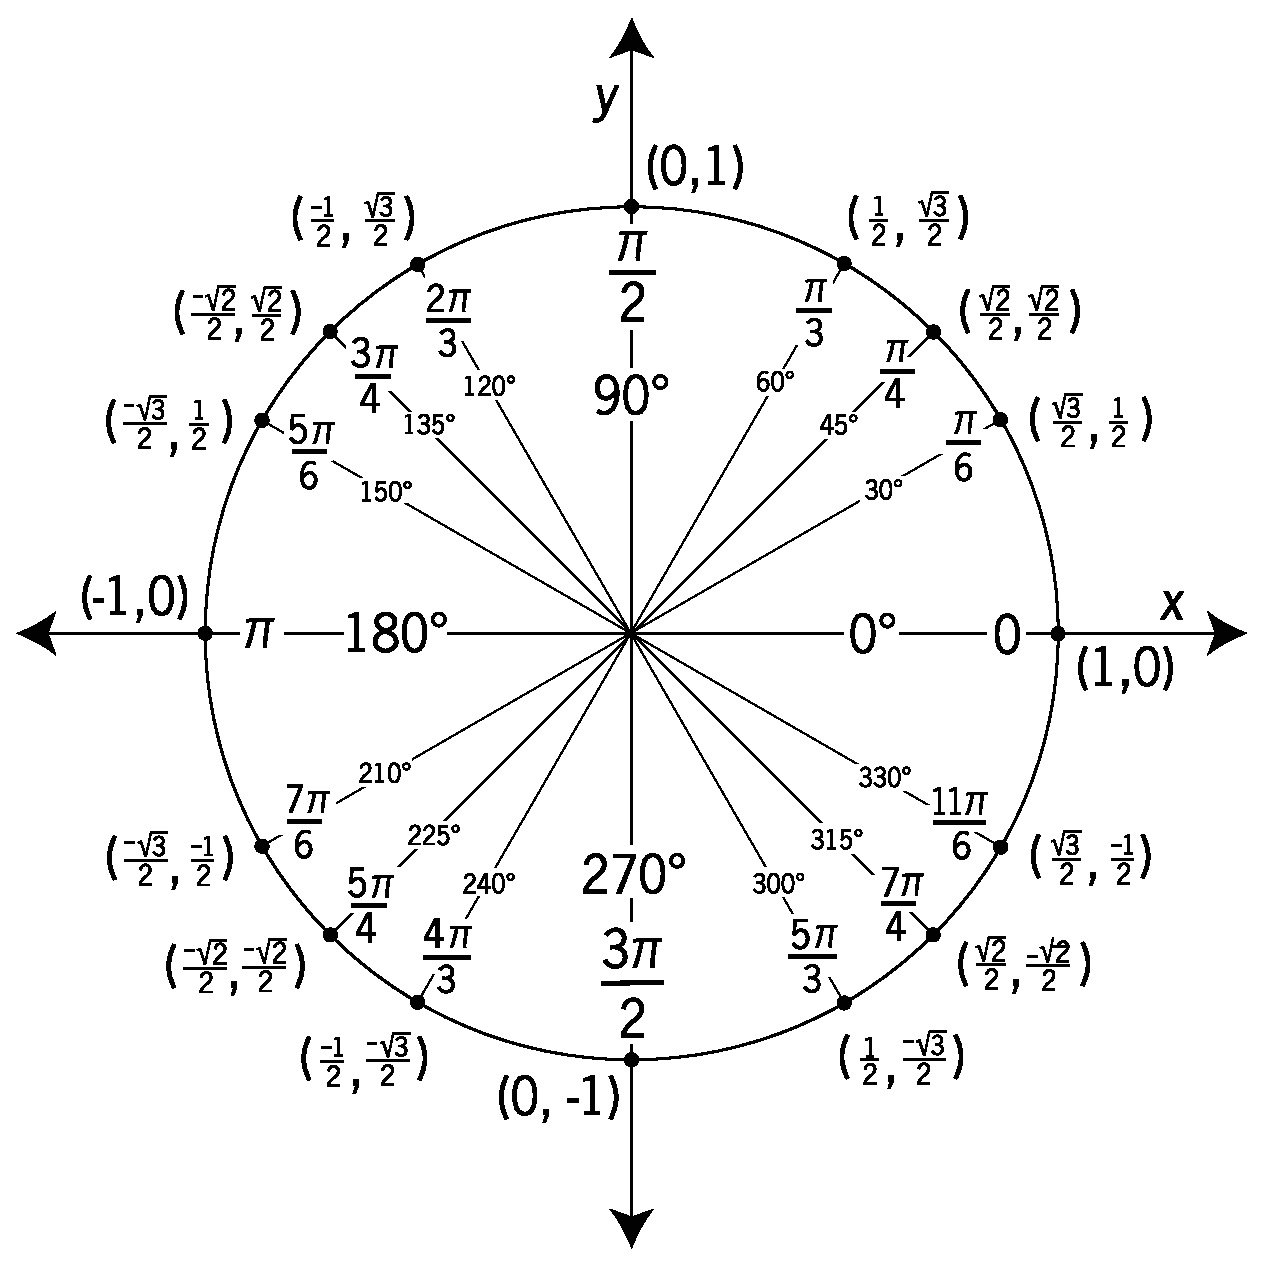
\includegraphics[width = \textwidth]{unit-circle7_43215}
Source: \url{https://etc.usf.edu/clipart/43200/43215/unit-circle7_43215.htm}

\subsection{Basic Trigonometry}
\begin{align*}
  sin(\theta) &= \frac{Opposite}{Hypotenuse}&
    cos(\theta) &= \frac{Adjacent}{Hypotenuse}&
    tan(\theta) &= \frac{Opposite}{Adjacent}\\
  &= \frac{y}{1} = y&
    &= \frac{x}{1} = x&
    &= \frac{y}{x}\\
  &&
    &&
    &= \frac{sin(\theta)}{cos(\theta)}\\
    \\
  csc(\theta) &= \frac{1}{sin(\theta)}&
    sec(\theta) &= \frac{1}{cos(\theta)}&
    cot(\theta) &= \frac{cos(\theta)}{sin(\theta)}
\end{align*}

\subsection{Pythagorean Theorem Identities}
\begin{gather*}
  sin^2 \theta + cos^2 \theta = 1\\
  tan^2 \theta + 1 = sec^2 \theta\\
  1 + cot^2 \theta = csc^2 \theta
\end{gather*}

\subsection{Half Angle Identities}
\begin{align*}
  cos(\frac{\theta}{2}) &= \pm \sqrt{\frac{1+cos(\theta)}{2}}&
    tan(\frac{\theta}{2}) &= \pm \sqrt{\frac{1-cos(\theta)}{2}}\\
  sin(\frac{\theta}{2}) &= \pm \sqrt{\frac{1-cos(\theta)}{2}}&
    &= \frac{sin(\theta)}{1+cos(\theta)}\\
  &&
    &= \frac{1-cos(\theta)}{sin(\theta)}
\end{align*}

\subsection{Double Angle Identities}
\begin{align*}
  sin (2\theta) &= 2sin\theta cos\theta\\
  cos (2\theta) &= cos^2 \theta - sin^2 \theta\\
  &= 2cos^2 \theta - 1\\
  &= 1 - 2sin^2 \theta\\
  tan (2\theta) &= \frac{2tan\theta}{1-tan^2 \theta}
\end{align*}

\subsection{Power Reduction Identities}
\begin{align*}
  sin^2\theta &= \frac{1-cos2\theta}{2}&
    csc^2\theta &= \frac{2}{1-cos2\theta}\\
  cos^2\theta &= \frac{1+cos2\theta}{2}&
    sec^2\theta &= \frac{2}{1+cos2\theta}\\
  tan^2\theta &= \frac{1-cos2\theta}{1+cos2\theta}&
    cot^2\theta &= \frac{1+cos2\theta}{1-cos2\theta}
\end{align*}

\section{Trigonometric Substitution}
\begin{center}
\begin{tabular}{c c c}
Expression & Substitution & Identity\\
$\sqrt{a^2 - b^2 x^2}$ & $x = \frac{a}{b} sin\theta$ & $1-sin^2 \theta = cos^2 \theta$\\
$\sqrt{a^2 + b^2 x^2}$ & $x = \frac{a}{b} tan\theta$ & $1-tan^2\theta = sec^2\theta$\\
$\sqrt{b^2 x^2 - a^2}$ & $x = \frac{a}{b} sec\theta$ & $sec^2\theta - 1 = tan^2 \theta$\\
\\
\end{tabular}
\end{center}

\begin{multicols}{2}

\section{Table of Basic Derivatives}
\begin{center}
\begin{tabular}{|c|c|}
\hline
$y$ & $\frac{dy}{dx}$\\
\hline
$C$ & $0$\\
\hline
$x$ & $1$\\
\hline
$ax^2 + bx + c$ & $2ax+b$\\
\hline
$x^n$ & $nx^{n-1}$\\
\hline
$x^{-1}, \frac{1}{x}$ & $-\frac{1}{x^2}$\\
\hline
$\sqrt{x}$ & $\frac{1}{2\sqrt{x}}$\\
\hline
$\sqrt[n]{x}$ & $\frac{1}{n\sqrt[n]{x^{n-1}}}$\\
\hline
$ln(x)$ & $\frac{1}{x}$\\
\hline
$log_a (x)$ & $\frac{1}{x ln(a)}$\\
\hline
$a^x$ & $a^x ln (a)$\\
\hline
$e^x$ & $e^x$\\
\hline
$sin(x)$ & $cos(x)$\\
\hline
$cos(x)$ & $-sin(x)$\\
\hline
$tan(x)$ & $\frac{1}{cos^2 x}, sec^2 x$\\
\hline
$cot(x)$ & $-\frac{1}{sin^2 x}, -csc^2 x$\\
\hline
$sec(x)$ & $tan(x) sec(x)$\\
\hline
$csc(x)$ & $-cot(x) csc(x)$\\
\hline
\end{tabular}
\end{center}

\columnbreak

\section{Table of Basic Integrals}

\begin{center}
\begin{tabular}{|c|c|}
\hline
$f(x)$ & $\int\limits f(x) dx = F(x) + C $\\
\hline
$x^\alpha$ & \multirow{2}{4em}{$\frac{x^{\alpha + 1}}{\alpha + 1} + C$}\\
  $\alpha \neq 0$ &\\
\hline
$sin(kx)$ & $-\frac{cos(kx)}{k} + C$\\
\hline
$cos(kx)$ & $\frac{sin(kx)}{k} + C$\\
\hline
$sec^2(kx)$ & $\frac{tan(kx)}{k} + C$\\
\hline
$csc^2(kx)$ & $-\frac{cot(kx)}{k+C}$\\
\hline
$e^{kx}$ & $\frac{e^{kx}}{k} + C$\\
\hline
$x^-1 , \frac{1}{x}$ & $ln|x| + C$\\
\hline
$\frac{1}{\sqrt{1-x^2}}$ & $sin^{-1} + C$\\
\hline
$\frac{1}{1+x^2}$ & $tan^{-1}x + C$\\
\hline
$a^{kx}$ & $\frac{1}{k ln a} a^{kx} + C$\\
\hline
$\frac{1}{\sqrt{a^2-x^2}}$ & $sin^{-1} \frac{x}{a} + C$\\
\hline
$\frac{1}{a^2 + x^2}$ & $\frac{1}{a} tan^{-1}(x/a) + C$\\
\hline
\end{tabular}
\end{center}

\end{multicols}

\section{Substitution Techniques}

\begin{multicols}{2}
\subsection{U Substitution}
\begin{gather*}
  \int\limits f(g(x)) g'(x) dx = \int\limits f(u) du = F(u) + C\\
  \text{where: } u = g(x), du =g'(x)
\end{gather*}
\hfill

\columnbreak

\subsection{Integration by Parts}
\begin{gather*}
  \int\limits f(x) g'(x) dx = f(x) g(x) - \int\limits g(x) f'(x) dx\\
  \int\limits u dv = u v - \int\limits v du\\
  \\
  \int\limits _a^b f(x)g'(x) = f(x)g(x) \Big| _a^b - \int\limits _a^b g(x)f'(x) dx
\end{gather*}
\end{multicols}

\section{Engineering Formulas}
\subsection{Spring Formulas}
\begin{gather*}
F = kx\\
W = \int\limits _a^b kx dx\\
\\
F = \text{Force (Newtons [N])}\\
k = \text{spring constant (Newton meters $^N/_m$)}\\
x = \text{change in distance (meters [m])}\\
W = \text{Work (Joules [J])}\\
a = \text{initial length (meters [m])}\\
b = \text{final length (meters [m])}
\end{gather*}

\subsection{Fluid Formulas}
\begin{gather*}
W = F \cdot d = \int\limits F dx\\
V = \pi r^2 h \text{(apply to cylinders)}\\
F = m \cdot a = V \cdot \rho\\
\\
W = \text{Weight ()}\\
F = \text{Force (Newtons [N])}\\
d = \text{distance (meters [d])}\\
m = \text{mass (meters$^3 [m^3]$)}\\
a = \text{acceleration (meters per second$^2$ [$^m/_{s^2}$])}\\
\rho = \text{Something}
\end{gather*}

\section{Method of Partial Fractions}
\begin{gather*}
  \int\limits \frac{P_n (x)}{Q_m (x)} dx \text{ when }m>n\\
  n \text{ and } m \text{ are defined as the degree of the numerator and the denominator.}
\end{gather*}

\subsection{Decomposition Types}
\begin{center}
\begin{tabular}{c c c}
Type & Factor Example & Decomposition\\
Linear Factor & $(x-4)$ & $\frac{A}{x-4}$\\
Repeated Linear Factor & $(x-4)^2$ & $\frac{A}{(x+4)} + \frac{B}{(x+4)^2}$\\
Quadratic Irreducible Factor & $(x^2+4)$ & $\frac{Ax+B}{x^2+4}$\\
Repeated Quadratic Irreducible Factor & $(x^2+4)^2$ & $\frac{Ax+B}{(x^2+4)} + \frac{Cx+D}{(x^2+4)^2}$
\end{tabular}
\end{center}

\pagebreak

\section{Additional Resources}
\textbf{Print}\\
Calculus Study Guide: \url{https://mt-jfk.com/ap-calculus-study-guide.pdf}\\
\\
\textbf{Video}\\
The Organic Chemistry Tutor: \url{https://www.youtube.com/channel/UCEWpbFLzoYGPfuWUMFPSaoA}\\
Black Pen Red Pen: \url{https://www.youtube.com/user/blackpenredpen}

\end{document}
